\documentclass[12pt]{article}
\usepackage[utf8]{inputenc}
\usepackage{float}
\usepackage{amsmath}

\usepackage[hmargin=3cm,vmargin=6.0cm]{geometry}
\topmargin=-2cm
\addtolength{\textheight}{6.5cm}
\addtolength{\textwidth}{2.0cm}
\setlength{\oddsidemargin}{0.0cm}
\setlength{\evensidemargin}{0.0cm}

\usepackage{tikz}
\usetikzlibrary{automata,positioning}

\begin{document}

\section*{Student Information } 
Full Name : Yaşar Cahit Yıldırım \\
Id Number : 2310647              \\



%------------------ QUESTION 1 ------------------
\section*{Answer 1}

\subsection*{a.}
  \begin{minipage}{0.3\textwidth}
    $$K = \{s, q_0, q_1, q_2, h\}$$
    $$\Sigma = \{a, b, \sqcup, \triangleright\}$$
    $$s = s$$
    $$H = \{h\}$$
  \end{minipage}
  and $\delta = $ \hspace{0.15cm}
  \begin{minipage}{0.7\textwidth}
    \begin{table}[H]
      \begin{tabular}{|lll|lll|}
        \hline
        $q  $ & $\sigma$ & $\delta(q, \sigma) $ & $q  $ & $\sigma        $ & $\delta(q, \sigma) $ \\ \hline
        $s  $ & $\Sigma$ & $(q_0, \rightarrow)$ & $q_2$ & $a             $ & $(q_2, \leftarrow) $ \\
        $q_0$ & $a     $ & $(q_1, \sqcup)     $ & $q_2$ & $b             $ & $(q_2, \leftarrow) $ \\
        $q_0$ & $b     $ & $(q_2, \sqcup)     $ & $q_2$ & $\sqcup        $ & $(h, b)            $ \\
        $q_0$ & $\sqcup$ & $(h, \sqcup)       $ & $s  $ & $\triangleright$ & $(s, \rightarrow)  $ \\
        $q_1$ & $a     $ & $(q_1, \leftarrow) $ & $q_0$ & $\triangleright$ & $(q_0, \rightarrow)$ \\
        $q_1$ & $b     $ & $(q_1, \leftarrow) $ & $q_1$ & $\triangleright$ & $(q_1, \rightarrow)$ \\
        $q_1$ & $\sqcup$ & $(h, a)            $ & $q_2$ & $\triangleright$ & $(q_2, \rightarrow)$ \\ \hline
      \end{tabular}
    \end{table}
  \end{minipage}

\subsection*{b.}
  
  \textbf{(i)}
  \begin{minipage}{0.4\textwidth}
    \begin{table}[H]
      \begin{tabular}{ll}
        $(s,\,\triangleright\sqcup\sqcup b\underline{a}b)$ & $\vdash_M\ (q_0,\,\triangleright\sqcup\sqcup ba\underline{b})$       \\
                                                          & $\vdash_M\ (q_2,\,\triangleright\sqcup\sqcup ba\underline{\sqcup})$  \\
                                                          & $\vdash_M\ (q_2s,\,\triangleright\sqcup\sqcup b\underline{a}\sqcup)$ \\
                                                          & $\vdash_M\ (q_2s,\,\triangleright\sqcup\sqcup \underline{b}a\sqcup)$ \\
                                                          & $\vdash_M\ (q_2s,\,\triangleright\sqcup\underline{\sqcup} ba\sqcup)$ \\
                                                          & $\vdash_M\ (h,\,\triangleright\sqcup\underline{b}ba\sqcup)$         
      \end{tabular}
    \end{table}
  \end{minipage}\\
  \vspace{1cm}
  \hspace{-0.3cm}
  \textbf{(ii)}
  \begin{minipage}{0.4\textwidth}
    \begin{table}[H]
      \begin{tabular}{ll}
        $(s,\,\triangleright a\underline{a}a)$ & $\vdash_M\ (q_0,\,\triangleright aa\underline{a})$      \\
                                               & $\vdash_M\ (q_1,\,\triangleright aa\underline{\sqcup})$ \\
                                               & $\vdash_M\ (q_1,\,\triangleright a\underline{a}\sqcup)$ \\
                                               & $\vdash_M\ (q_1,\,\triangleright \underline{a}a\sqcup)$ \\
                                               & $\vdash_M\ (q_1,\,\underline{\triangleright} aa\sqcup)$ \\
                                               & $\vdash_M\ (q_1,\,\triangleright \underline{a}a\sqcup)$
      \end{tabular}
    \end{table}
  \end{minipage}
  \begin{minipage}{0.4\textwidth}
    After this, machine will never stop and will repeat last two configurations.
  \end{minipage}\\
  \textbf{(iii)}
  \begin{minipage}{0.4\textwidth}
    \begin{table}[H]
      \begin{tabular}{ll}
        $(s,\,\triangleright \underline{a}\sqcup bb)$ & $(q_0,\,\triangleright a\underline{\sqcup}bb)$ \\
                                                      & $(h,\,\triangleright a\underline{\sqcup}bb)$  
      \end{tabular}
    \end{table}
  \end{minipage}
  \newpage


%------------------ QUESTION 2 ------------------
\section*{Answer 2}

  $$(\triangleright\underline{\sqcup} babc)\vdash(\triangleright\sqcup\underline{b}abc)\vdash^4(\triangleright\sqcup babc\underline{\sqcup})\vdash(\triangleright\sqcup bab\underline{c})\vdash^2(\triangleright\sqcup babc\underline{\sqcup})\vdash(\triangleright\sqcup babc\sqcup\underline{b})$$
  $$\vdash(\triangleright\sqcup babc\sqcup\underline{c})\vdash^2(\triangleright\sqcup babc\sqcup c\underline{\sqcup})\vdash(\triangleright\sqcup babc\sqcup c\sqcup\underline{b})$$\\

  \qquad Machine takes a step to the right. It looks at the symbol on its head.(Let it be variable $a$) It goes right until it finds a blank symbol. It takes a step back to the left and checks if the symbol there is a $c$. If it is not a $c$ it halts, else(let this $c$ be called variable $b$) it takes a step to the right, writes blank symbol there, takes a step to the right. It then writes the $a$ there, and overwrites it with $b$. Takes a step to right, writes blank symbol, takes one step to right and finally writes $a$.


%------------------ QUESTION 3 ------------------
\section*{Answer 3}

  \subsection*{a.}
    $$\{w : w \in \{a,b\}^*\}$$

  \subsection*{b.}
    Let $N_x(s)$ be the number of $x$ symbols in string $s$.
    $$f(w) = a^nb^m \text{ where } w \in \{a, b\}^*, N_a(w) = n, N_b(w) = m$$


%------------------ QUESTION 4 ------------------
\section*{Answer 4}

  \begin{center}
    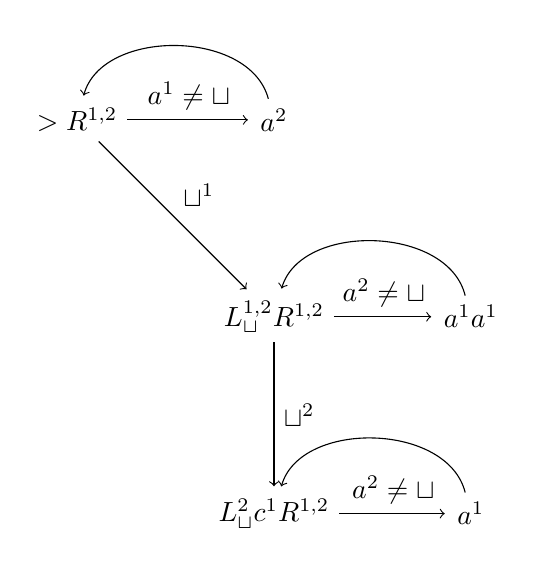
\begin{tikzpicture}[shorten >= 1pt, node distance=2.5cm, on grid, auto]
      \node (0)              {$> R^{1,2}$};
      \node (1) [right=of 0] {$a^2$};
      \node (2) [below=of 1] {$L_\sqcup^{1,2}R^{1,2}$};
      \node (3) [right=of 2] {$a^1a^1$};
      \node (4) [below=of 2] {$L_\sqcup^2c^1R^{1,2}$};
      \node (5) [right=of 4] {$a^1$};

      \path[->]
        (0) edge node {$a^1\neq\sqcup$} (1)
        (0) edge node {$\sqcup^1$} (2)
        (1) edge [bend right=75] node {} (0)
        (2) edge node {$a^2\neq\sqcup$} (3)
        (2) edge node {$\sqcup^2$} (4)
        (3) edge [bend right=75] node {} (2)
        (4) edge node {$a^2\neq\sqcup$} (5)
        (5) edge [bend right=75] node {} (4);
    \end{tikzpicture}
  \end{center}
  \newpage


%------------------ QUESTION 5 ------------------
\section*{Answer 5}

  \begin{center}
    \begin{tikzpicture}[shorten >= 1pt, node distance=4cm, on grid, auto]
      \node (0)              {$> R^{1,2}$};
      \node (1) [right=of 0] {$a^2$};
      \node (2) [below=of 1] {$L_\sqcup^{1,2}R^{1,2}$};
      \node (3) [right=of 2] {$a^1R^1a^1\sqcup^2R_\sqcup^2L^2$};
      \node (4) [right=of 3] {$a^1$};

      \path[->]
        (0) edge node {$a^1\neq\sqcup$} (1)
        (0) edge node {$\sqcup^1$} (2)
        (1) edge [bend right=75] node {} (0)
        (2) edge node {$a^2\neq\sqcup$} (3)
        (3) edge node {$a^2\neq\sqcup$} (4)
        (4) edge [bend right=75] node {} (2);
    \end{tikzpicture}
  \end{center}


%------------------ QUESTION 6 ------------------
\section*{Answer 6}

  \subsection*{a.}
    $$\delta\;:\;\big((K-H) \times (\Sigma-\{\triangleright\}) \mapsto K\times((\Sigma-\{\triangleright\}) \cup \{\downarrow\})\big) \cup \big((K-H) \times \{\triangleright\} \mapsto K\times(\Sigma-\{\triangleright\})\big)$$

  \subsection*{b.}
    \qquad To preserve determinism, there should only be one transition possible at a given time and configuration. So in order to add $e$-transitions to TM, we should consider a different approach.

    \qquad For $e$-transitions to be achieved, a state $p$'s all transitions must have the same right hand side, i.e. $(p, a) \mapsto (q, X)$ for all $p$ where $q\in K$ and $X$ is any action. Only then, we can replace all these transitions with only $(p, e) \mapsto (q, X)$.

    \qquad After this flexibility provided, our $\Sigma$ from the left hand side of $\delta$ mapping should be changed with $\Sigma \cup \{e\}$.

  \subsection*{c.}
    Let $(q_1, f_1w_1)$ and $(q_2, f_2w_2)$ be configurations of the machine. Then $$(q_1, f_1w_1) \vdash (q_2, f_2w_2)$$ if and only if, for some $X \in \Sigma\cup\{\downarrow\}$, $\delta(q_1, f_1) = (q_2,  X)$, and either,
    \begin{itemize}
      \item $X \in \Sigma, f_1=f_2, w_2 = w_1X$
      \item $X = \downarrow, w_1 = f_2w_2$.
    \end{itemize}
  
  \newpage

  \subsection*{d.}

    $$M = \{K, \{a,b,c,\triangleright, \#\}, \delta, q_0, \{halt\}\}$$

    \begin{itemize}
      \item $Y\rightarrow X$ means that if front is $Y$ then do $X$.
      \item $b,c,\# \rightarrow b,c,\#$ means that push the symbol that you have seen. ($b,c,\#$)
      \item $pop$ state which $q_6$ and $q_7$ transites to, goes to $q_0$ and pops one element whatever the front is, i.e. $q_0$'s are the same state. (Hard to draw.)
    \end{itemize}
    \vspace*{2cm}

    \tikzset{every loop/.style={min distance=10mm,looseness=10}}
    \hspace{-1.5cm}
    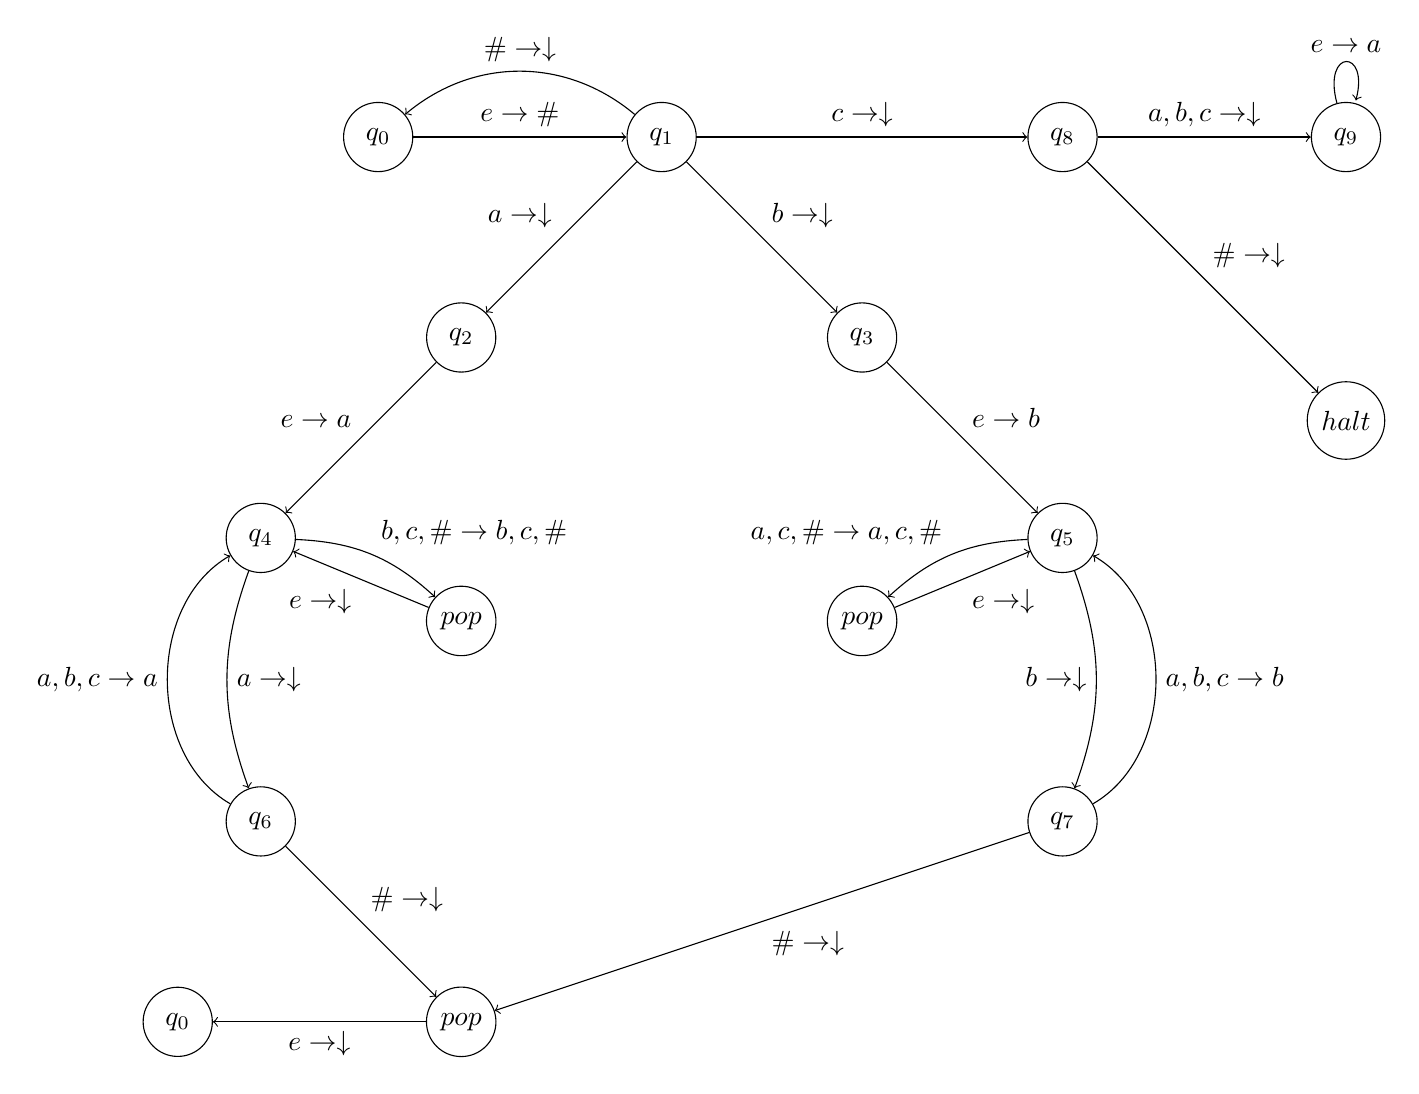
\begin{tikzpicture}[node distance=3.6cm,on grid,auto] 
      \node[state] (q0)                     {$q_0$};
      \node[state] (q1) [right of=q0]       {$q_1$};
      \node[state] (q2) [below left of=q1]  {$q_2$};
      \node[state] (q4) [below left of=q2]  {$q_4$};
      \node[state] (q3) [below right of=q1] {$q_3$};
      \node[state] (q5) [below right of=q3] {$q_5$};
      \node[state] (q6) [below of=q4]       {$q_6$};
      \node[state] (q7) [below of=q5]       {$q_7$};
      \node[state] (q8) [above right of=q3] {$q_8$};
      \node[state] (q9) [right of=q8]       {$q_9$};
      \node[state] (p)  [below right of=q6] {$pop$};
      \node[state] (qq) [left of=p]         {$q_0$};
      \node[state] (p4) [above right of=q6] {$pop$};
      \node[state] (p5) [above left of=q7]  {$pop$};
      \node[state] (h)  [below of=q9]       {$halt$};

      \path [->]
      (q0) edge                         node {$e\rightarrow\#$} (q1)
      (q1) edge                         node {$c\rightarrow\downarrow$} (q8)
      (q8) edge                         node {$\#\rightarrow\downarrow$} (h)
      (q8) edge                         node {$a,b,c\rightarrow\downarrow$} (q9)
      (q9) edge [loop above]            node {$e\rightarrow a$} ()
      (q1) edge [swap]                  node {$a\rightarrow\downarrow$} (q2)
      (q1) edge [swap, bend right = 40] node {$\#\rightarrow\downarrow$} (q0)
      (q2) edge [swap]                  node {$e\rightarrow a$} (q4)
      (q4) edge [bend left = 20]        node {$b,c,\#\rightarrow b,c,\#$} (p4)
      (p4) edge                         node {$e\rightarrow\downarrow$} (q4)
      (q4) edge [bend right = 20]       node {$a\rightarrow\downarrow$} (q6)
      (q6) edge [bend left = 60]        node {$a,b,c\rightarrow a$} (q4)
      (q6) edge                         node {$\#\rightarrow\downarrow$} (p)
      (q1) edge                         node {$b\rightarrow\downarrow$} (q3)
      (q3) edge                         node {$e\rightarrow b$} (q5)
      (q5) edge [swap, bend right = 20] node {$a,c,\#\rightarrow a,c,\#$} (p5)
      (p5) edge [swap]                  node {$e\rightarrow\downarrow$} (q5)
      (q5) edge [swap, bend left = 20]  node {$b\rightarrow\downarrow$} (q7)
      (q7) edge [swap, bend right = 60] node {$a,b,c\rightarrow b$} (q5)
      (q7) edge                         node {$\#\rightarrow\downarrow$} (p)
      (p)  edge                         node {$e\rightarrow\downarrow$} (qq);

    \end{tikzpicture}
  \newpage


%------------------ QUESTION 7 ------------------
\section*{Answer 7}

  \subsection*{a.}
    An insert-delete TM is a quintuple $(K, \Sigma, \delta, s, H)$ where
    \begin{itemize}
      \item $K$ is a finite set of states,
      \item $\Sigma$ is an alphabet contaning the left end symbol $\triangleright$,
      \item s $\in K$ is the initial state,
      \item $H\subseteq K$ is the set of halting states,
      \item $\delta$ is the transition function where it is defined as 
    \end{itemize}
    $\delta\;:\;(K-H) \times (\Sigma\cup\{e\}-\{\triangleright\})^2 \mapsto K\times(\Sigma\cup\{e,\uparrow\}-\{\triangleright\})^2 \cup () - ((K-H) \times \{e\}^2 \mapsto K\times\{e\}^2)$

  \subsection*{b.} 
    \qquad The configuration for an insert-delete TM is a member of $K \times \triangleright\Sigma^*$. We can only work with the first symbol after $\triangleright$ and the last so no need to specify.

  \subsection*{c.}
    \qquad Let $(q_1, f_1w_1r_1)$ and $(q_2, f_2w_2r_2)$ be configurations of the machine. Then $(q_1, f_1w_1r_1) \vdash (q_2, f_2w_2r_2)$ iff., for some $a,b \in \Sigma\cup\{\uparrow\}$, $\delta(q_1, l_1, r_1) = (q_2, a, b)$ and after $a, b$ actions to $a_1, r_1$, the tape became $f_2w_2r_2$. If $a\text{ or }b\in\Sigma$ then machine inserts at that position, otherwise if $a \text{ or } b = \uparrow$ it deletes from that position.

  \subsection*{d.}
    \qquad Can an insert-delete TM be obtained from a TM? We do only finite number of operations in one step so it can be obtained. We can think of insert-delete TM as a two headed single tape TM such that one head is at the beginning and other at the end of the string. Allowing this TM to have exact functionality as insert-delete TM shows that insert-delete TM can be obtained from a conventional TM.

    \qquad Can a TM be obtained from an insert-delete TM? Since we know where the end of the string is, we can have unrestricted access to a specific memory place by marking techniques and state configurations. So since we have infinite amount of memory and unrestricted access to it, we can do whatever turing machines can do.


  \newpage
%------------------ QUESTION 8 ------------------
\section*{Answer 8}

  \qquad $G = (V, \Sigma, R, S)$ where
  \begin{center}
    $V=\{S,a,L,R,A,P,H,T\}$\\
    $\Sigma=\{a\}$\\
    \begin{align*}
      R=\{ & S \rightarrow LAPR\\\\
           & HA \rightarrow aACH\\
           & Ha \rightarrow aH\\
           & HC \rightarrow aCH\\
           & HR \rightarrow AAPR\\\\
           & aP \rightarrow Pa\\
           & AP \rightarrow PA\\
           & CP \rightarrow PC\\
           & LP \rightarrow LH\\
           & PR \rightarrow T\\\\
           & aT \rightarrow Ta\\
           & AT \rightarrow Ta\\
           & CT \rightarrow Ta\\
           & LT \rightarrow \epsilon\}.
    \end{align*}
  \end{center}


%------------------ QUESTION 9 ------------------
\section*{Answer 9}

  \qquad Let $L_A$ be $L_1L_2$ so that $L=L_A\cap L_3$. We know that $L_1$ and $L_2$ are recursively enumerable so there are some TM's $M_1$ and $M_2$'s that semidecides them respectively.

  \qquad In order to build a TM $M_A$ that semidecides $L_A$ we can use the high level definition as following:\\

  \qquad On input word $w$:
  \begin{itemize}
    \item Nondeterministically split the word $w$ as $w_1w_2$.
    \item Run $M_1$ on $w_1$.
    \item Run $M_2$ on $w_2$.
    \item If both $M_1$ and $M_2$ halts(accepts), halt(accept).
  \end{itemize}

  \qquad Also, since we know $L_3$ is recursively enumerable, there is a TM $M_3$ that semidecides it. We now can construct a TM $M$ that semidecides $L$ with the high level definition as following:\\

  \qquad On input word $w$:
  \begin{itemize}
    \item Run $M_A$ on $w$.
    \item If $M_A$ halts(accepts), run $M_3$ on $w$.
    \item If $M_3$ halts(accepts), halt(accept).
  \end{itemize}

  \qquad It is now proved by defined semideciding TM $M$ that $L$ is recursively enumerable.





















\end{document}